\documentclass[a4paper]{scrartcl}
\usepackage[T1]{fontenc}
\usepackage[utf8]{inputenc}
\usepackage{amsmath,amssymb,amsfonts}
\usepackage{xcolor}
\usepackage{tikz}
\usetikzlibrary{arrows, arrows.meta, fit, positioning, shapes, backgrounds}
\usepackage{pgfplots}
\pgfplotsset{compat=1.18}
\usetikzlibrary{decorations.pathreplacing}
\usetikzlibrary{svg.path}
\usetikzlibrary{calc}
\usepackage{tikz-cd}
\pgfplotsset{compat=1.15}
\usetikzlibrary{patterns,patterns.meta}
\usetikzlibrary{arrows}

\newcommand{\Dow}{\mathcal{D}}

\newcommand{\eps}{\varepsilon}

\begin{document}

    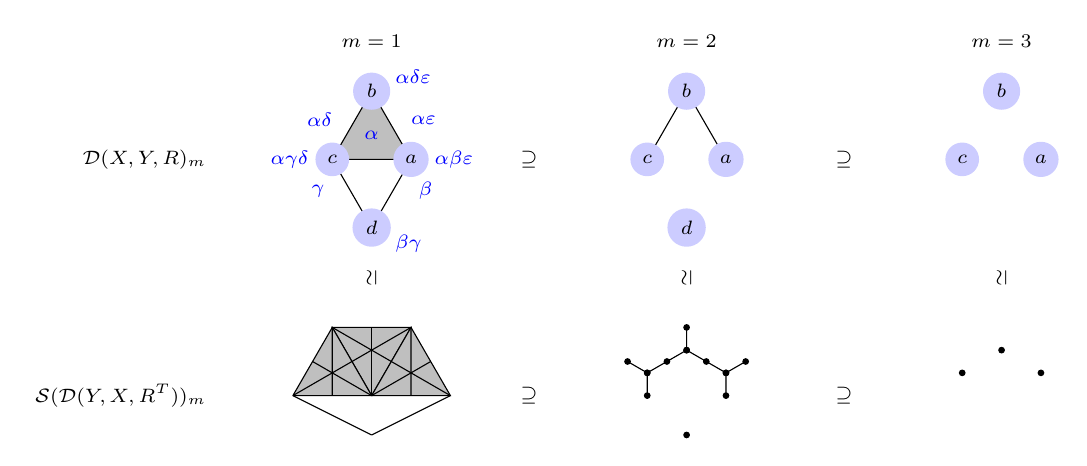
\begin{tikzpicture}
    \scriptsize

    \node[left,align=flush right] at (-2,0){$\Dow(X,Y,R)_m$};
    \node[left,align=flush right] at (-2,-3){$\mathcal{S}(\Dow(Y,X,R^T))_m$};


        \node at (0,1.5) {$m=1$};


    %%%%%%%%%%%%%%%%%%TOP LEFT PANEL%%%%%%%%%%%%%%%%%%%%%%%%
    %centered at (0,0)

        \draw[] (0.5,0) -- 
                (0,{-sqrt(3)/2}) node[circle, fill=blue!20] {$d$} -- 
                (-0.5,0);
        \draw[fill=gray!50] (0.5,0) node[circle, fill=blue!20] {$a$} -- 
                            (0,{sqrt(3)/2}) node[circle, fill=blue!20](b) {$b$} --
                            (-0.5,0) node[circle, fill=blue!20](c) {$c$} -- 
                            (0.5,0);

        \node[blue, right] at(0.7,0){$\alpha\beta\eps$}; 
        \node[blue, left] at(-0.7,0){$\alpha\gamma\delta$};
        \node[blue, above right] at(0.2,{sqrt(3)/2}){$\alpha\delta\eps$};
        \node[blue, below right] at(0.2,{-sqrt(3)/2}){$\beta\gamma$};

        \node[blue, left] at(-0.4,0.5){$\alpha\delta$};
        \node[blue, right] at(0.4,0.5){$\alpha\eps$};
        \node[blue, left] at(-0.5,-0.4){$\gamma$};
        \node[blue, right] at(0.5,-0.4){$\beta$};

        \node[blue] at(0,0.3){$\alpha$};

        \node at (0,-1.5) {\rotatebox{90}{$\simeq$}};

        %%%%%%%%%%%%%%%%%BOTTOM LEFT PANEL%%%%%%%%%%%%%%%%%%
        %centered at (0,-3)

        \draw (-1,-3) to (0,-3.5);
        \draw (0,-3.5) to (1,-3);
        \draw[fill=gray!50] (0,-3)  -- 
                            (-0.5,{sqrt(3)/2-3})  -- 
                            (0.5,{sqrt(3)/2-3}) -- 
                            (0,-3);
        \draw[fill=gray!50] (0,-3)  -- 
                            (0.5,{sqrt(3)/2-3})  -- 
                            (1,-3)  -- 
                            (0,-3);
        \draw[fill=gray!50] (-1,-3)  -- 
                            (-0.5,{sqrt(3)/2-3})  -- 
                            (0,-3) -- 
                            (-1,-3);
        \draw (-1,-3) -- 
              (0.5,{sqrt(3)/2-3}) -- 
              (0.5,-3);
        \draw (1,-3) -- 
              (-0.5,{sqrt(3)/2-3}) -- 
              (-0.5,-3);
        \draw (-0.75,{sqrt(3)/4-3}) -- 
              (0,-3) -- 
              (0.75, {sqrt(3)/4-3});
        \draw (0,{sqrt(3)/2-3}) -- (0,-3);


        \node at (4,1.5) {$m=2$};


        %%%%%%%%%%%%%%%%%%TOP MIDDLE PANEL%%%%%%%%%%%%%%%%%%%%
        %centered at (4,0)

        \node at (2,0) {$\supseteq$};

        \draw[] (4.5,0) node[circle, fill=blue!20] {$a$} -- 
                (4,{sqrt(3)/2}) node[circle, fill=blue!20] {$b$} -- 
                (3.5,0) node[circle, fill=blue!20] {$c$};
        \node[circle, fill=blue!20] at (4,{-sqrt(3)/2}) {$d$};


        \node at (4,-1.5) {\rotatebox{90}{$\simeq$}};


        \node at (2,-3) {$\supseteq$};


        %%%%%%%%%%%%%%%BOTTOM MIDDLE PANEL%%%%%%%%%%%%%%%%%%%%%%%%%
        %centered at (4,-3)
        \draw[fill] (4,-3.5) circle (1pt);
        \draw[fill=black] (4,{sqrt(3)/2-3}) circle[fill, radius = 1pt]  -- 
                          (4,{sqrt(3)/3-3}) circle[fill, radius = 1pt];
        \draw[fill=black] (3.5,{sqrt(3)/6-3}) circle[fill, radius = 1pt]
                        -- (3.75,{sqrt(3)/4-3}) circle[fill, radius = 1pt] 
                        -- (4,{sqrt(3)/3-3}) circle[fill, radius = 1pt] 
                        -- (4.25,{sqrt(3)/4-3}) circle[fill, radius = 1pt] 
                        -- (4.5,{sqrt(3)/6-3}) circle[fill, radius = 1pt];
        \draw[fill=black] (3.25,{sqrt(3)/4-3}) circle[fill, radius = 1pt] -- 
                          (3.5,{sqrt(3)/6-3}) circle[fill, radius = 1pt]-- 
                          (3.5,-3)circle[fill, radius = 1pt];
        \draw[fill=black] (4.5,-3) circle[fill, radius = 1pt] -- 
                          (4.5,{sqrt(3)/6-3})circle[fill, radius = 1pt] -- 
                          (4.75, {sqrt(3)/4-3})circle[fill, radius = 1pt];


        \node at (8,1.5) {$m=3$};



        \node at (6,0) {$\supseteq$};

        %%%%%%%%%%%%%%TOP RIGHT PANEL%%%%%%%%%%%%%%%%%%
        %centered at (8,0)
        \node[circle, fill=blue!20] at (7.5,0) {$c$};
        \node[circle, fill=blue!20] at (8,{sqrt(3)/2}) {$b$};
        \node[circle, fill=blue!20] at (8.5,0) {$a$};


        \node at (8,-1.5) {\rotatebox{90}{$\simeq$}};


        \node at (6,-3) {$\supseteq$};

        %%%%%%%%%%%%%%%%BOTTOM RIGHT PANEL%%%%%%%%%%%%%%%
        %centered at (8,-3)
        \draw[fill] (7.5, {sqrt(3)/6-3}) circle (1pt);
        \draw[fill] (8, {sqrt(3)/3-3}) circle (1pt);
        \draw[fill] (8.5, {sqrt(3)/6-3}) circle (1pt);

\end{tikzpicture}

\end{document}